\documentclass[11pt,letterpaper]{article}

\addtolength{\oddsidemargin}{-.875in}
\addtolength{\evensidemargin}{-.875in}
\addtolength{\textwidth}{1.75in}

\addtolength{\topmargin}{-.875in}
\addtolength{\textheight}{1.75in}

\usepackage[utf8]{inputenc}
\usepackage{caption} % for table captions
\usepackage{amsmath} % for multi-line equations and piecewises
\DeclareMathOperator{\sign}{sign}
\usepackage{graphicx}
\usepackage{relsize}
\usepackage{xspace}
\usepackage{verbatim} % for block comments
\usepackage{subcaption} % for subfigures
\usepackage{enumitem} % for a) b) c) lists
\newcommand{\Cyclus}{\textsc{Cyclus}\xspace}%
\newcommand{\Cycamore}{\textsc{Cycamore}\xspace}%
\newcommand{\deploy}{\texttt{d3ploy}\xspace}%
\newcommand{\Deploy}{\texttt{D3ploy}\xspace}%
\usepackage{tabularx}
\usepackage{color}
\usepackage{multirow}
\usepackage{float}
\usepackage[acronym,toc]{glossaries}
\newacronym{ANL}{ANL}{Argonne National Laboratory}
\newacronym{B4C}{B4C}{boron carbide}
\newacronym{BC}{BC}{boundary condition}
\newacronym{BOC}{BOC}{beginning of equilibrium cycle}
\newacronym{BSD}{BSD}{Berkeley Software Distribution}
\newacronym{BWR}{BWR}{Boiling Water Reactor}
\newacronym{CAISO}{CAISO}{California ISO}
\newacronym{CEA}{CEA}{Commissariat a l'Energie Atomique}
\newacronym{CFD}{CFD}{computational fluid dynamics}
\newacronym{CO2}{CO$_2$}{carbon dioxide}
\newacronym{CR}{CR}{control rod}
\newacronym{CRP}{CRP}{Coordinated Research Project}
\newacronym{CZP}{CZP}{Cold Zero Power}
\newacronym{DCC}{DCC}{depressurized conduction cool-down}
\newacronym{DOE}{DOE}{Department of Energy}
\newacronym[\glslongpluralkey={degrees of freedom}]{DoF}{DoF}{degree of freedom}
\newacronym{EOC}{EOEC}{end of equilibrium cycle}
\newacronym{FCEV}{FCEV}{Fuel Cell Electric Vehicle}
\newacronym{FDM}{FDM}{Finite Difference Method}
\newacronym{FEM}{FEM}{Finite Element Method}
\newacronym{FVM}{FVM}{Finite Volume Method}
\newacronym{FSV}{FSV}{Fort St. Vrain}
\newacronym[\glslongpluralkey={greenhouse gases}]{GHG}{GHG}{greenhouse gas}
\newacronym{GRS}{GRS}{Gesellschaft für Anlagen und Reaktorsicherheit}
\newacronym{H2}{H$_2$}{hydrogen}
\newacronym{He}{He}{helium}
\newacronym{HFP}{HFP}{Hot Full Power}
\newacronym{HPCC}{HPCC}{high pressure conduction cool-down}
\newacronym{HTE}{HTE}{High-Temperature Electrolysis}
\newacronym{HTGR}{HTGR}{High-Temperature Gas-Cooled Reactor}
\newacronym{HTR}{HTR}{High Temperature Reactor}
\newacronym{HTTR}{HTTR}{High Temperature Test Reactor}
\newacronym{HZDR}{HZDR}{Helmholtz-Zentrum Dresden-Rossendorf}
\newacronym{IAEA}{IAEA}{International Atomic Energy Agency}
\newacronym{icap}{iCAP}{Illinois Climate Action Plan}
\newacronym{INL}{INL}{Idaho National Laboratory}
\newacronym{IPyC}{IPyC}{inner pyrolytic carbon}
\newacronym{JFNK}{JFNK}{Jacobian-Free Newton-Krylov}
\newacronym{KAERI}{KAERI}{Korea Atomic Energy Research Institute}
\newacronym{Keff}{K$_{eff}$}{multiplication factor}
\newacronym{LBP}{LBP}{Lumped Burnable Poison}
\newacronym{LGPL}{LGPL}{Lesser GNU Public License}
\newacronym{LOCA}{LOCA}{loss of coolant accident}
\newacronym{LPCC}{LPCC}{low pressure conduction cool-down}
\newacronym{LTE}{LTE}{Low-Temperature Electrolysis}
\newacronym{LWR}{LWR}{Light Water Reactor}
\newacronym{MC}{MC}{Monte Carlo}
\newacronym{MHTGR}{MHTGR}{Modular High-Temperature Gas-Cooled Reactor}
\newacronym{MOC}{MOC}{middle of equilibrium cycle}
\newacronym{MOOSE}{MOOSE}{Multi-physics Object-Oriented Simulation Environment}
\newacronym{MPI}{MPI}{Message Passing Interface}
\newacronym{MSR}{MSR}{Molten Salt Reactor}
\newacronym{MTD}{MTD}{Champaign-Urbana Mass Transit District}
\newacronym{NEA}{NEA}{Nuclear Energy Agency}
\newacronym{NEM}{NEM}{Nodal Expansion Method}
\newacronym{NGNP}{NGNP}{Next Generation Nuclear Power}
\newacronym{NRC}{NRC}{Nuclear Regulatory Commission}
\newacronym{NSC}{NSC}{Nuclear Science Committee}
\newacronym{OECD}{OECD}{Organisation for Economic Co-operation and Development}
\newacronym{OPyC}{OPyC}{outer pyrolytic carbon}
\newacronym{ORNL}{ORNL}{Oak Ridge National Laboratory}
\newacronym{OS}{OS}{Operator-Splitting}
\newacronym{PBMR}{PBMR}{Pebble Bed Modular Reactor}
\newacronym{PDE}{PDE}{Partial Differential Equation}
\newacronym{PMR}{PMR}{Prismatic Modular Reactor}
\newacronym{PV}{PV}{photovoltaics}
\newacronym{RSC}{RSC}{Reserve Shutdown Control}
\newacronym{RSD}{RSD}{Relative Standard Deviation}
\newacronym{SD}{SD}{Standard Deviation}
\newacronym{SI}{SI}{Sulfur-Iodine}
\newacronym{SiC}{SiC}{silicon carbide}
\newacronym{SMR}{SMR}{Small Modular Reactor}
\newacronym{SNU}{SNU}{Seoul National University}
\newacronym{SOEC}{SOEC}{Solid Oxide Electrolysis Cells}
\newacronym{TIP}{TIP}{transverse integration procedure}
\newacronym{TRISO}{TRISO}{Tristructural Isotropic}
\newacronym{UIUC}{UIUC}{University of Illinois at Urbana-Champaign}
\newacronym{UNIST}{UNIST}{Ulsan National Institute of Science and Technology}
\newacronym{UK}{UK}{United Kingdom}
\newacronym{UMICH}{UMICH}{University of Michigan}
\newacronym{US}{US}{United States}
\newacronym{VHTR}{VHTR}{Very High Temperature Gas Cooled Reactor}
%\newacronym{<++>}{<++>}{<++>}
%\newacronym{<++>}{<++>}{<++>}

\definecolor{bg}{rgb}{0.95,0.95,0.95}
\newcolumntype{b}{X}
\newcolumntype{f}{>{\hsize=.15\hsize}X}
\newcolumntype{s}{>{\hsize=.5\hsize}X}
\newcolumntype{m}{>{\hsize=.75\hsize}X}
\newcolumntype{r}{>{\hsize=1.1\hsize}X}
\usepackage{titling}
\usepackage[hang,flushmargin]{footmisc}
\renewcommand*\footnoterule{}
\usepackage{tikz}
\usepackage{array}
\usepackage{booktabs,mathptmx,siunitx}
\sisetup{input-symbols = {()},  % do not treat "(" and ")" in any special way
         group-digits  = false} % no grouping of digits

\usetikzlibrary{shapes.geometric,arrows}
\tikzstyle{process} = [rectangle, rounded corners,
minimum width=1cm, minimum height=1cm,text centered, draw=black,
fill=blue!30]
\tikzstyle{arrow} = [thick,->,>=stealth]

\graphicspath{}

\begin{document}

\section{Prismatic \gls{HTGR} Neutronic Solvers}

Nowadays there are several codes to solve the neutronics of prismatic \glspl{HTGR}.
Most of these codes rely on one of the following methods: stochastic transport (Monte Carlo), deterministic transport, or deterministic diffusion.
We focus our interest in the last method.
% If time permits work on a brief description of the Monte Carlo and deterministic transport maybe.
% Why? Deterministic diffusion solvers have lower computational requirements than other methods reference ??
% The utilization of the Monte Carlo codes is unattractive because of the tremendous problem size and the need for a large number of neutron histories \cite{lee_status_2006}.
% It is one of the simplest means to solve neutron transport problems \cite{leppanen_development_2007}.
% Here I say the following
% Deterministic diffusion methods are computationally cheaper than the other methods.
% This characteristic makes it a good candidate for coupled calculations.

The history of deterministic diffusion solvers begins in the late 1950s with the application of the \gls{FDM} to the analysis of \glspl{LWR}.
In \gls{FDM}, mesh spacings are usually of the order of the diffusion length.
When solving large multi-dimensional problems, this feature causes the mesh points to reach intractable numbers \cite{lewis_finite_1986}.
The computational expense of these calculations motivated the generation of more computationally efficient techniques \cite{lawrence_progress_1986}.
Although there are substantial overlaps, the most common techniques fall into two broad categories: nodal methods and \gls{FEM}.

% NODAL
FLARE \cite{delp_flare_1964} is a three-dimensional \gls{BWR} simulator and it is representative of the first generation of nodal schemes.
Such approach used adjusted parameters to match actual operating data or the results of more accurate calculations.
Most of these methods were implementations of the so-called 1.5 group theory.
A second generation of nodal schemes derived spatial coupling relationships by applying the \gls{TIP}.
Integrating the multi-dimensional diffusion equation over directions transverse to each coordinate axis, such procedure obtains equivalent one-dimensional equations \cite{lawrence_progress_1986}.
This approach proved to be highly efficient and accurate in Cartesian geometries.

In 1981, a formulation based on the \gls{NEM} first demonstrated the feasibility of nodal methods in hexagonal geometries \cite{duracz_nodal_1981}.
Nevertheless, this method would introduce non-physical singular terms that required the utilization of discontinuous polynomials.
This motivated the development of more effective formulations.
The code HEXNOD, introduced in 1988 \cite{wagner_three-dimensional_1989}, is an example of such formulations.
This algorithm uses the \gls{TIP} and, in contrast to the \gls{NEM}, solves the resulting differential equation analytically.
The article demonstrated the accuracy of the method by comparison with the \gls{FDM} and Monte Carlo calculations for a few benchmark problems.

Another example of more effective methods is the code HEXPEDITE \cite{fitzpatrick_hexpedite_1992}.
The HEXPEDITE approach uses the \gls{TIP} to derive a pseudo-one-dimensional equation.
The resulting differential equation is solved analytically.
The difference from HEXNOD is that, HEXPEDITE uses a different coupling scheme that is simpler and more efficient.
Different works \cite{fitzpatrick_hexpedite_1992}\cite{fitzpatrick_developments_1995} on the HEXPEDITE methodology tested the approach against the \gls{NEM} and the \gls{FDM}.
These studies established HEXPEDITE’s superiority in terms of accuracy and runtime.
HEXPEDITE's use still prevailed until recently in the analysis of \glspl{HTGR}.
In 2010, \gls{INL} conducted a study \cite{ortensi_deterministic_2010-1} in which they compared HEXPEDITE's results against the diffusion codes JAR, CITATION, and CRONOS2, and the Monte Carlo codes MCNP5 and Serpent.

Other examples of nodal diffusion codes whose use prevailed until the present are DIF3D \cite{lawrence_dif3d_1983} and PARCS \cite{downar_parcs_2004}.
DIF3D has several solution options such as the diffusion \gls{FDM}, diffusion \gls{NEM} based on \gls{TIP}, and the VARIANT nodal transport method.
% VARIANT: variational nodal \cite{palmiotti_variant_1995}
PARCS has several solution options as well, such as a diffusion \gls{FDM}, diffusion \gls{NEM} based on \gls{TIP}, P$_{N}$ transport methods, and the multigroup transport Simplified P$_3$ with \gls{FDM} and \gls{NEM} discretizations.

% from ortensi_deterministic_2010-1 and wang_modified_2018
Nodal methods solve quite coarse meshes for approximate solutions.
This characteristic makes the method efficient.
On the other hand, the method does not provide detailed point-wise accurate solutions \cite{kang_finite_1973}.

Additionally, nodal methods are applicable for the nodes of a specific shape on which the nodal method was derived.
The application to complex problems is not flexible as different geometries require the integration over different coordinate systems.
This lack of flexibility limits the applications of nodal methods to regular geometries only.

% FEM
The \gls{FEM} is a well-established method in applied mathematics and engineering.
\gls{FEM} is a numerical technique for finding approximate solutions to \glspl{PDE} by deriving their weak or variational form.
Most applications make \gls{FEM} preferable due to its flexibility in the treatment of curved or irregular geometries.
Also, the use of high order elements attains higher rates of convergence \cite{cavdar_finite_2004}.
The first prototype engineering application of \gls{FEM} was in the field of structural engineering and dates back to 1956.
In the successive years, \gls{FEM} became the most extensively used technique in almost every branch of engineering.
\glspl{FEM} have several advantages over the nodal methods.
It provides flexibility in the geometry definition, a firm mathematical basis, ease in extension to multi-group application, and high computational efficiency \cite{lee_development_2008}.

In 1973, an article by Kang et al. \cite{kang_finite_1973} described the first application of \gls{FEM} to the neutron diffusion theory.
The main motivation for this development was the impractical application of the \gls{FDM} to three-dimensional problems.
In this early work, the author compared different \gls{FEM} approaches to the \gls{FDM} in one-dimensional and two-dimensional problems.
The studies showed a higher order of convergence achieved by the \gls{FEM}.

Throughout the last four decades many codes have use the \gls{FEM} to solve the diffusion equation.
Some of the most recent codes are CRONOS2 \cite{lautard_cronos_1990}, CAPP \cite{lee_development_2011}, and Rattlesnake \cite{wang_rattlesnake_2019}.
The list of \gls{FEM} diffusion solvers is more extensive, but here we focus on the best documented codes in the open literature.
We also emphasize that most of the \gls{FEM} diffusion solvers for \glspl{HTGR} were born as \gls{LWR} analysis codes.

% CRONOS
\gls{CEA} developed CRONOS2 \cite{lautard_cronos_1990} as part of the SAPHYR system.
It allows for solving steady-state and transient multi-group calculations taking into account thermal-hydraulic feedback effects.
The code solves either the diffusion equation or the transport equation by means of the SN method.
In 2008, Damian et al. \cite{damian_vhtr_2008} conducted a study aimed at understanding the physical aspects of the annular core and the passive safety features of a standard block type \gls{HTGR}.
For such study, the authors developed the code suit NEPTHIS/CAST3M.
NEPHTIS uses a transport-diffusion calculation scheme that relies on CRONOS2.

% CAPP
In 2008, \gls{KAERI} published an article \cite{lee_development_2008} that presented the code CAPP.
The code's purposes are to conduct steady state core physics analysis, core depletion analysis, and core transient analysis.
The article validated the code with two benchmark problems.
First, the IAEA PWR benchmark problem for two cases, a 2D exercise and a 3D exercise.
Second, Phase I Exercise 1 of the OECD/NEA PBMR-400 benchmark problem.
The calculations of both problems used different number of elements and different orders of shape functions.

In 2011, Lee et al. published an article \cite{lee_development_2011} in which they extended the functionalities of the CAPP code to prismatic \glspl{HTGR}.
To take into account the thermal feedback, the authors developed a simplified thermal-hydraulics analysis tool.
To validate their model, the authors solved a two-dimensional model of the PMR-200 at \gls{BOC}.
The PMR-200 is a pre-conceptual reactor that \gls{KAERI} has designed.
They validation compared the results against the HELIOS\cite{stammler_helios_1998} results.
The results showed good accuracy.
Moreover, the authors implemented a depletion solver based on the one-group flux determined by the neutron flux solver.
The authors validated the depletion solver by calculating the multiplication factor as a burnup function of a single fuel block of the PMR-200.
They compared the results against the results obtained with HELIOS.
The maximum error was less than 200 pcm.

Tak et al. \cite{tak_cappgamma_2016} developed a coupling between the CAPP code and the GAMMA+ code \cite{lim_gamma_2006}.
GAMMA+ is a system code for thermal-hydraulics analysis and system transients.
In such study, the authors applied the coupled code to study the steady-state performance of the PMR-200.
They conducted several studies, such as a core depletion calculation, a core depletion calculation with critical control rod position search, and the analysis of the bypass flow effects on the coupled calculations.
Their results revealed that neglecting the bypass flow decreases the active core temperatures and, consequently, the multiplication factor increases by approximately 300 pcm.

A recent article by Yuk et al. \cite{yuk_time-dependent_2020} added to CAPP the capability to conduct transient analyses.
This capability solves the time dependent neutron diffusion equation with the \gls{FEM}.
The main motivation behind this feature is to enable the code to conduct reactivity insertion accidents.
Additionally, the article introduces a new method to resolve the control rod cusping effect \cite{joo_resolution_1984}.
To take into account the thermal feedback, the authors developed a simplified thermal-hydraulics analysis tool.
The new method integrates over partially rodded computation nodes and they called it iPRN.
To test its accuracy, the authors conducted two exercises with several methods that reduce the rod cusping effect.
The authors used the mesh reconstruction method to obtain the reference results, as such method eliminates the rod cusping effect by updating the mesh at every time step.
The iPRN method showed a higher accuracy than the other methods.
To test the new transient capabilities, they analyzed two control rod ejection scenarios and compared the results to those of CAPP/GAMMA+ coupled code.
Both codes showed similar results.

% Proghorn and Rattlesnake
RattleSnake \cite{wang_rattlesnake_2019} is the MOOSE \cite{gaston_moose_2009} based application for simulating the transport equation.
\gls{INL} has initially developed the Pronghorn code to model gas cooled pebble bed reactors.
The MOOSE neutronics kernel library Yak incorporated the neutron diffusion models originally in Pronghorn \cite{strydom_inl_2013}.
Currently, RattleSnake is the primary tool for solving the linearized Boltzmann neutron transport equation within MOOSE and relies heavily on the use of Yak.
There are a variety of solvers available under RattleSnake including low-order multigroup diffusion, spherical harmonics transport, and discrete ordinates transport all solved with the \gls{FEM}.
% Both RattleSnake and Pronghorn yielded the same exact results when using the continuous \gls{FEM} multigroup diffusion option in RattleSnake.

% j_ortensi_relap-7_2012 j_ortensi_initial_2012
In 2012, \gls{INL} published a work \cite{j_ortensi_initial_2012} that coupled Pronghorn and RELAP-7 \cite{andrs_relap-7_2012}.
Pronghorn solved the coupled equations that define the neutron diffusion, fluid flow, and heat transfer in a three-dimensional model.
RELAP-7 is a MOOSE-based system code and it solves the one-dimensional continuity, momentum, and energy equations for a compressible fluid.
It was responsible for modeling the plant system layout, which included the hot and cold ducts, the helium circulator, and the steam generator.
% This study integrated PRONGHORN and RELAP-7 with the operator split approach (or loose coupling) where each application used an independent mesh.
To test the coupling, the integrated system carried out the OECD/NEA MHTGR-350 Benchmark \cite{oecd_nea_coupled_2020}.
The original benchmark provides a set of 26 neutron energy group and temperature dependent cross sections.
To simplify the debugging, the authors collapsed the 26 groups into two groups.
Although using two groups reduces the accuracy of the model, the lower number of groups decreases the calculation time by a factor of ten or more.
In this study, a two-dimensional cylindrical model replaced the three-dimensional geometry defined by the benchmark.
The testing of the integrated system included 2 stages: (1) both codes working independently underwent several convergence studies, and (2) the codes solved the steady-state problem in an integrated manner.
The authors concluded that the coupling between Pronghorn and RELAP-7 was successful.

% strydom_inl_2013
In 2013, \gls{INL} conducted the OECD/NEA MHTGR-350 Benchmark \cite{strydom_inl_2013} without further simplifications.
The \gls{INL} team solved Exercise 1 of Phase I using INSTANT-P1 \cite{wang_krylov_2011}, Pronghorn, and RattleSnake.
% They also solved exercises 2 and 3 using RELAP5-3D and PHISICS/RELAP5-3D code suit.
INSTANT is transport solver that relies on the spherical harmonics discretization of angles.
The results for Pronghorn and RattleSnake are identical.
By modifying the cross-sections, INSTANT-P1 returns the diffusion solution.
Its results were within 30 pcm from Pronghorn and RattleSnake results.
All presented results exhibited good agreement with the benchmark results.

\subsection{Energy group structure analysis}

% yuk_time-dependent_2020
% The authors recommend homogenizing the group constants using at least 10 energy groups.

% Number of energy groups impact over the calculations
The longer neutron mean free path in \glspl{HTGR} compared to \gls{LWR} increases the spectral interactions between elements.
For this reason, \gls{HTGR} analyses require more energy groups than conventional \gls{LWR} analyses.
\gls{ANL} directed a study \cite{lee_status_2006} to compare the accuracy of nodal diffusion calculations employing different energy group structures to generate the homogenized cross-sections.
The cross-section homogenization used the code DRAGON and the diffusion calculations utilized the code DIF3D.
For the study, the ANL team implemented a one-dimensional fuel-reflector model in which they used 4, 7, 8, 14, and 23 energy groups.
They also used alternative energy group structures for the same number of groups.
For simplicity, the authors used the homogenized fuel compact model.
They generated all the cross-sections at 300 K.
One of their conclusions was that the number of energy groups should be more than 4, and 7 or more would be sufficient for uranium fueled \glspl{HTGR}.
Another conclusion was that the accuracy of the diffusion calculation is sensitive to the energy group boundaries.
% Mention something about the metrics of the study? To asses the accuracy, they compared the multiplication factor.

% han_sensitivity_2008
Han's MS thesis \cite{han_sensitivity_2008} focused on the selection of energy groups for the reactor analysis of the \gls{PBMR}.
The author used the code COMBINE6 \cite{grimesey_combinepc-portable_1994} for cross section generation and the Penn State nodal diffusion code NEM \cite{bandini_three-dimensional_1990} for the reactor analysis.
The author compared the results against reference results obtained with the code MCNP5 \cite{rsicc_computer_code_collection_mcnp5_2003}.
To simplify the set up, the model used uniformly distributed isotopes in the fuel.
The study performed the calculations at two different temperatures: 300 and 1000 K.
To arrive at an optimal group structure, the author compared many series of combinations of group structures using a trial and error strategy.
One of the conclusion of this work agrees with previous bibliography \cite{gulf_oil_company_nuclear_1973} \cite{duderstadt_nuclear_1976} on the fact that the energy spectrum is key to yield an accurate description of a nuclear reactor using a few groups.

ANL's study is helpful for setting up properly nodal diffusion calculations for an \gls{HTGR}.
Although the conclusions could be extrapolated to \gls{FEM} diffusion solvers, such study might be valuable.
ANL's team conducted the study at 300 K, which is not in the operational range of any \glspl{HTGR}.
In the contrary, Han's thesis included an analysis at 1000 K, and his results showed that the temperature changes have a non-negligible impact.
Additionally, ANL's study used the simplified model of the homogenized fuel compact.
Han's highlighted that homogenized fuel models of the \gls{PBMR} underestimate criticality calculations.
In 2015, \gls{INL} presented their results \cite{strydom_results_2015} for an \gls{IAEA} Coordinated Research Program \cite{tyobeka_htgr_2011} and showed that the homogenization of the compact material underestimates notably the eigenvalue.
On the other hand, the open literature has not investigated the impact of such simplification over the homogenized cross sections.


\section{Prismatic \gls{HTGR} Thermo-Hydraulics}

% sort of motivation
Thermal-hydraulic calculations enable the correct design of \glspl{HTGR}.
The ability to predict the maximum fuel temperature at steady-state is of paramount importance to succeed in such task.
We emphasize this statement in the case hydrogen production is desirable.
Efficient hydrogen production requires higher coolant temperatures, which in turn increases the temperature of the fuel and the reactor pressure vessel.

% sort of intro to simplified models
The complex geometry of the hexagonal fuel assembly requires elaborate numerical calculations for obtaining accurate evaluations.
Thermal-hydraulic studies for early \glspl{HTGR} consisted mainly of support calculations for \gls{NRC} safety analysis reports.
The analyses employed sets of independent codes that relied on simplistic approximations.
Simplified models are helpful to understand some basic aspects of prismatic \glspl{HTGR} and have the advantage to reduce the computational expense of the calculations.

% shenoy_htgr_1974
General Atomics \cite{shenoy_htgr_1974} developed the first set of simplistic codes.
The following list introduces and summarizes some of these codes and their features:

\begin{itemize}
\item FLAC: It determines the coolant flow distribution in the coolant channels and gaps.
It solves the one-dimensional momentum equation for incompressible flow and the continuity equations for mass and energy.

\item POKE: It determines the coolant mass flow, coolant temperature, and fuel temperature distribution.
It solves the steady-state mass and momentum conservation equations for parallel channels.

\item DEMISE: It determines the steady-state three-dimensional temperature distribution in a standard element.
It solves the temperature in a network model.

\item TAC-2D: It is a general purpose two-dimensional thermal analysis code.
It solves the two-dimensional heat conduction equation.
\end{itemize}

Several studies have used these codes.
% macdonald_ngnp_2003
For example, \gls{INL} conducted in 2003 a design study \cite{macdonald_ngnp_2003} in support to the \gls{NGNP} project.
The objective of such study was to investigate options for the NGNP that increased the coolant temperature, with the lowest possible inlet temperature, and the highest overall core power.
The authors conducted several parametric studies whose reference reactor was the GT-MHR \cite{general_atomics_gas_1996}.
Using the code POKE, they evaluated two major design modifications: reducing the bypass flow and better controlling the inlet coolant flow distribution.
Reducing the bypass flow fraction from 20 to 10$\%$ reduces the peak fuel temperatures by about 50$^{\circ}$C.
Controlling the inlet flow distribution has a stronger effect.
Other studies focused on the dimensions of the reactor and their impact on the maximum fuel temperature.
Using the computer codes POKE and TAC2D, the authors investigated taller and higher power reactor cores.
The investigation included a 10-block-high 600 MWt, a 12-block-high 720 MWt, and 14-block-high 840 MWt.

Among the simplified approaches we differentiate the flow network model, the equivalent cylindrical model, and the unit cell model.
% flow network model
% reza_design_2006
Using the network analysis tool RELAP5-3D/ATHENA \cite{inl_relap5-3dathena_2005}, Reza et al. \cite{reza_design_2006} conducted a thermal hydraulic study of the GT-MHR.
Reza et al. increased the reactor outlet temperature to enable hydrogen production.
Additionally, they evaluated alternative coolant inflow paths in an attempt to reduce the reactor vessel temperatures.
After finding an optimal configuration, they evaluated the maximum temperatures in the fuel and the reactor vessel during the \gls{LPCC} and the \gls{HPCC} events.

% equivalent cylindrical model
% no_multi-component_2007
An example of codes using the equivalent cylindrical approach is GAMMA \cite{no_multi-component_2007}.
The code’s main objective is the modeling of the air ingress event following a LOCA.
Following the depressurization of helium in the core, there exists the potential for air to enter the core through the break and oxidize the in-core graphite structure.
The oxidation of graphite leads to exothermic chemical reactions and, thus, it is a major concern.
The GAMMA code solves heat conduction, fluid flow, chemical reactions, and multi-component molecular diffusion.
The code couples the solid and gas equations using the porous media model.
Together with the multi-dimensional analysis feature, GAMMA has a one-dimensional analysis capability for  modeling a flow network.

% takada_core_2004
Takada et al. \cite{takada_core_2004} carried out another study using the flow network and the equivalent cylindrical model.
Focusing on the \gls{HTTR}, they developed a thermal-hydraulic design code.
The code used the flow network analysis code FLOWNET \cite{maruyama_verification_1988} for calculating the coolant flow and temperature distributions.
The code TEMDIM \cite{maruyama_verification_1988} solved the fuel temperatures using the equivalent cylindrical model.
Finally, the authors validated the calculation scheme by comparing its results with the experimental data from the \gls{HTTR}.

% unit cell model
% nakano_conceptual_2008
Nakano et al. \cite{nakano_conceptual_2008} studied different fuel assembly configurations using several simplistic approximations.
For determining the fuel temperature, they used the TAC-2D code.
A previous nuclear analysis calculated the power density.
And a previous study calculated the flow distribution using the code FLOWNET.
The fuel temperature calculation used the equivalent cylindrical model for a hot channel unit cell.
However, the asymmetry of the unit cell configuration makes the temperature distribution asymmetric in the graphite block.
The equivalent cylindrical model fails to capture this behavior.

% in_three-dimensional_2006
In 2006, In et al. \cite{in_three-dimensional_2006} conducted a more detailed analysis using a three-dimensional model of the unit cell in the hot-spot of an \gls{HTGR}.
The objective of the study was to predict the maximum fuel temperature at steady-state.
The analysis focused on the GT-MHR 600 at \gls{EOC}.
The CFD code CFX 10 \cite{ansys_inc_cfx_2006} calculated the three-dimensional temperature profile.
In such a study, the results showed that the maximum fuel temperature surpassed the design limits and the authors propose a countermeasure accordingly.

% more detailed calculations
Such simplified approaches are helpful to understand some basic aspects of prismatic \glspl{HTGR} but they may affect the temperature distribution.
More detailed thermal-hydraulic evaluations were rare in the open literature until the last 15 years.

% cioni_3d_2005
Cioni et al. \cite{cioni_3d_2006} presented an article in 2005 in which they conducted three-dimensional simulations of fuel assemblies of an \gls{HTGR}.
The objective of the study was to investigate an emergency situation due to the blocking of cooling channels in the core.
They used the \gls{CFD} code Trio_U \cite{bieder_priceles_2000} to carry out the analysis.
The numerical scheme solved the three-dimensional conduction equation in the solid coupled to the one-dimensional thermal-hydraulic equations of the coolant.
In the preliminary work, the authors conducted a study of the influence of the bypass flow on the maximum coolant and fuel temperature.
Another preliminary study analyzed the consequences of two different blocking in a portion of a fuel assembly.
A central blockage exhibits a stronger influence over the maximum temperatures of the assembly compared to a peripheral blockage.
At last, they investigated two configurations.
First, six fuel elements surrounded the fuel element with the blockage.
Second, five fuel elements and one reflector element surrounded it.
The results suggested that the blockage increases the temperature on the blocked fuel assembly only and it does not affect the surrounding elements due to the bypass flow.
The results also showed that the fuel temperature surpassed the design limits, and that the reactor operators should counteract these effects with active systems.

% simoneau_three-dimensional_2007
Simoneau et al. \cite{simoneau_three-dimensional_2007} analyzed the transient behavior of an \gls{HTGR} during the \gls{DCC} and \gls{HPCC} event.
The CFD code STAR-CD \cite{computational_dynamics_limited_star-cd_2004} performed the calculations.
The code solved conductive, convective, and radiation heat transfer in a 30$^{\circ}$ section of the core and reactor vessel.
To accommodate the different spatial scales, the code uses the porous media model to represent the coolant flow and the prismatic fuel blocks.
The model does not resolve the boundary layer and the use of coefficients prescribe the solid-fluid heat transfer and pressure drop across the core.
The authors validated their model against explicit calculations using a single fuel block.
One of their results shows that the maximum temperature in the \gls{HPCC} event is lower than in the \gls{DCC} event.
However, the extra convective heat transfer causes a thermal stratification in the surrounding air, causing higher temperatures in the upper reactor structures.

% tak_numerical_2008
In 2008, an article by Tak et al. \cite{tak_numerical_2008} conducted  a three-dimensional \gls{CFD} analysis on a typical prismatic \gls{HTGR} fuel column.
The commercial code CFX 11 \cite{ansys_incorporated_cfx_2006} performed the calculations.
The fuel column under study was from the PMR-600, a pre-conceptual reactor that \gls{KAERI} has designed and whose reference design is the GT-MHR.
The study considered a one-twelfth section of the fuel due to its symmetry.
The model determined the coolant distribution using the one-dimensional thermal-hydraulic equations.
Such coolant distribution served as input to the CFD code.
Nevertheless, the friction in the channels is dependent on the viscosity which is highly dependent on the temperature.
Therefore, obtaining the mass flow rates from a separate solver may introduce errors \cite{sato_computational_2010}.
As mentioned earlier, the unit cell model may introduce errors in the maximum temperature prediction.
In order to asses the accuracy of the unit cell model, the authors compared the CFD results against the unit cell model results.
The unit cell model does not consider the bypass flow between assemblies or the radial power distribution within the fuel assembly.
Tak et al. conducted a parametric study which analyzed the impact of the bypass gap size on the maximum fuel temperature.
By increasing the bypass gap, the maximum fuel temperature grows.
The results of this study indicate that the accuracy of the unit cell worsens for larger gaps.
Another study imposed different radial peaking factors for the different fuel channels.
Such a study showed the effects of considering a non-flat radial power distribution.
The authors considered a radial power distribution that did not have a strong impact on the maximum fuel temperature.

% sato_computational_2010
Another article \cite{sato_computational_2010} carried out \gls{CFD} calculations of a typical prismatic \gls{HTGR} with the commercial code FLUENT \cite{fluent_inc_fluent_2006}.
Their model considered a one-twelfth section of the fuel column of the GT-MHR.
The authors conducted parametric studies changing several factors, such as bypass gap-width, turbulence model, axial heat generation profile, and geometry changes due to irradiation.
Their most relevant results show the presence of bypass flow causes a large lateral temperature gradient in the block.
Large temperature gradients cause excessive thermal stresses which raise potential structural issues.
The authors compared the results from different turbulence models: $k \sim \varepsilon$ and $k \sim \omega$.
The $k \sim \omega$ model predicted bulk temperatures that are considerably lower than those from the $k \sim \varepsilon$ model.
The differences went up to 49$^{\circ}$C.
The overall mass flow rate is about 10$\%$ greater for the $k \sim \omega$ model.
The study suggested that these turbulence models need more verification against prismatic \gls{HTGR} experiments.
Another study analyzed the effect of considering different peak radial factors.
Such consideration introduced variations of the maximum fuel temperature of up to 160 $^{\circ}$C.
Their last study focused on the effects of the graphite dimensional changes on the temperature profile.
The shrunk column showed considerably lower temperatures in the fuel.

% travis_thermalhydraulics_2013
In spite of the recent developments in CFD tools, a detailed full core explicit analysis for a prismatic \gls{HTGR} still requires a tremendous computational expense.
This requirement is mostly due to the three-dimensional CFD simulation of the coolant flow.
Travis et al. \cite{travis_thermalhydraulics_2013} developed a method to compute full core thermal-hydraulic analyses of \glspl{HTGR}.
The article presented a simplified method that reduces the computational time and memory requirements while maintaining accurate results.
The method solves the three-dimensional heat conduction in the solid and the one-dimensional thermal-hydraulic equations in the channels.
The fluid one-dimensional approximation avoids finer meshes near the walls as well as turbulence conservation equations \cite{tak_development_2014}.
The validation of the method analyzed a fuel column and compared the results to those of a three-dimensional CFD simulation.
The CFD simulation used the commercial software STAR-CCM+ \cite{cd-adapco_star-ccm_2012}.
The new computational scheme reduced the computation time to a 2.5\% of the time required by the three-dimensional CFD simulation.
The new method provided good predictions of the temperature distribution and the axial variation of the helium bulk temperature.
However, it failed to resolve properly the velocity and temperature distribution within the boundary layer.
Overall, the method showed good accuracy, and less than a 2\% difference to the three-dimensional CFD simulation.

% tak_practical_2012 / tak_development_2014
Tak et al. \cite{tak_practical_2012} \cite{tak_development_2014} developed CORONA, which uses a practical method for the whole core analysis.
The code intends to combine the accuracy from CFD tools and the light computational expense of system analysis codes.
The method solves the three-dimensional heat conduction equation in the solid and the one-dimensional thermal-hydraulic equations in the fluid.
In order to enhance practicability, the code adopts a basic unit cell concept, which eliminates an elaborate grid generation process.
The basic unit cell concept is an extension of the traditional unit cell method, which uses a single triangular unit cell.
This method considers various shapes of unit cells as well as the heat transfer between them.
The method provides a way for fast generating computational grids for modeling the solid regions.
To validate the new code, the authors compared the results using CORONA against the results using the commercial code CFX and experimental results.
The results of the verification and validation studies showed that the CORONA code provides reasonably accurate results.

% end of section
CFD techniques allow to compute the detailed temperature profile over local models.
The fine mesh requirement imposes high computational costs for a whole core CFD analysis, restricting the use of such methods.
However, a whole-core thermal analysis has many advantages over local models.
In general, the problem set up includes more accurate boundary conditions.
Without whole-core modeling, the mass flow distributions in local models are average values of the core flow rate instead of their exact value \cite{huning_novel_2016}.
This leads to under predicted fuel temperatures for the assemblies with a lower flow rate than the average.
Additionally, a coupled analysis with a reactor physics code requires a full core model \cite{tak_practical_2012}.

% this might appear in a summary of the chapter: see travis_thermalhydraulics_2013 / tak_practical_2012 / tak_development_2014 
% The fine mesh requirement for a whole core CFD analysis restricts the use of such methods.
% Most of the CFD studies limit their application to the local behavior of a fuel column.
% The alternative for an explicit whole-core analysis are system codes that use simplified models.
% However, the simplification of the geometries reduces the fuel block temperature resolution.
% The present method intends to overcome the difficulties in CFD calculation as well as in system calculations.
% The computational expense of a solid heat conduction equation is much less than that of fluid conservation equations in CFD analyses .
% This requirement is mostly due to the three-dimensional CFD simulation of the coolant flow.
% The methodology provides good predictions of the global parameters such as the three-dimensional spatial temperature distribution and the axial variation of the helium bulk temperature \cite{travis_thermalhydraulics_2013}.
% The fluid one-dimensional approximation avoids finer meshes near the walls as well as turbulence conservation equations \cite{tak_development_2014}.

\section{Coupled Neutronics/Thermal-Hydraulics}

---> From here

% sort of intro ?
% I should add somewhere around here something on the coupled simulations:
% In order to consider the interaction between the neutronics and thermal-fluids behavior, a coupled analysis is necessary /cite{tak_cappgamma_2016}.

% damian_vhtr_2008
Damian et al. \cite{damian_vhtr_2008} conducted a study aimed at understanding the physical aspects of the annular core and the passive safety features of a standard block type \gls{HTGR}.
They performed the analysis of various geometrical scales: fuel cell and fuel column located at the core hot spot, 2D and 3D core configurations including the coupling between neutronics and thermal-hydraulics.

The first part of the assessment concerns thermal calculations on steady-state core configurations.
Such study used CAST3M \cite{studer_cast3marcturus_2007} code considering a 3D thermal coupled with 1D hydraulic modeling.
The authors conducted a parametric study on the maximum fuel temperature by modifying the fuel compact and the fuel element geometries.
An annular fuel compact and the reduction of the number of fuel compacts in the outer ring yielded the best performance.

The second part of the assessment used a 2D core configuration using the transport code APOLLO2 \cite{sanchez_apollo2_1999} to minimize the radial power peaking factor.
The analysis included the variation of various parameters such as fuel enrichment, fuel loading, and the fuel management scheme.
The fuel enrichment variation had the strongest impact.

The last part of the study analyzed a 3D core model using the coupled codes NEPTHIS \cite{cavalier_presentation_2005} and CAST3M/Arcturus.
The study varies several design parameters and studies the impact on the power distribution.
Such parameters are the helium by-pass fraction, average power density, core geometry, reflector materials, and fuel loading strategy.
The codes NEPTHIS and CAST3M/Arcturus calculate the neutronics and the thermal-hydraulics, respectively.
NEPHTIS uses a transport-diffusion calculation scheme that relies on APOLLO2 and the diffusion code CRONOS2 \cite{lautard_cronos_1990}.
The CRONOS2 code solves either the diffusion equation or the even parity transport equation, and it uses a \gls{FDM} or a \gls{FEM} discretization.
The CAST3M/Arcturus model uses a two-level approach.
On the first level, the porous media model solves the homogenized system and the coolant.
On the second level, the CAST3M code solves the thermal-hydraulics on the homogenized geometry.
Some of the conclusions of this last part of the study were that although the reduction of the bypass fraction decreases the maximum fuel temperature, the average reflector temperature rises.
Another conclusion showed that using magnesium oxide for the reflector material yields lower temperatures for both normal operation and transients.

% CAPP
In 2011, Lee et al. published an article \cite{lee_development_2011} in which they extended the functionalities of the CAPP code to prismatic \glspl{HTGR}.
To take into account the thermal feedback, the authors developed a simplified thermal-hydraulics analysis tool.
The thermal-hydraulics solver divides fuel column in six triangular prisms.
Each of them hosts a representative coolant channel.
Solving the energy equation, the code calculates the axial coolant temperature distribution.
After calculating the coolant temperature, a two-dimensional conduction model solves the moderator and fuel compact temperatures.
By means of a TRISO particle conduction model, the model obtains the fuel temperature.
Finally, a three-dimensional conduction model based on the \gls{FDM} allows for solving the reflector temperature.
% The cross-sections are a function of burnup, moderator temperature, and fuel temperature.
To validate their model, the authors solved a two-dimensional model of the PMR-200 at \gls{BOC}.
The PMR-200 is a pre-conceptual reactor that \gls{KAERI} has designed.
They compared the results against the results obtained with HELIOS.
The results showed good accuracy.
Moreover, the authors implemented a depletion solver based on the one-group flux determined by the neutron flux solver.
% Cross sections generated with HELIOS.
The authors validated the depletion solver by calculating the multiplication factor as a burnup function of a single fuel block of the PMR-200.
They compared the results against the results obtained with HELIOS.
The maximum error was less than 200 pcm.

% tak_coupled_2016
Tak et al. tak_development_2014
This work laid the foundation for the neutronics/thermal-hydraulics coupling of DeCART (citation) and CORONA discussed in the following section (?)

Tak et al. \cite{tak_coupled_2016} developed a neutronics/thermal-hydraulics coupled code using DeCART \cite{kaeri_decart_2007} and CORONA.
To validate the new code, the authors conducted the OECD/NEA MHTGR-350 benchmark.
The main objectives of the calculation are to validate the code and also identify technical challenges for future development.

DeCART is a whole-core neutron transport code and it is responsible for calculating the power distribution and the fast neutron fluence.
CORONA calculates the temperature distribution.

The authors present an interesting analysis where they compared the results from the coupled simulation and the stand-alone simulations.
The difference in the multiplication factor was as high as 2597 pcm.
The axial offset and maximum fuel temperature exhibited significant differences as well.
Such result highlights the importance of the integration of both neutronics and thermal-hydraulic solvers.

% tak_cappgamma_2016
Another article \cite{tak_cappgamma_2016} introduces a coupling between the CAPP code and the GAMMA+ code \cite{lim_gamma_2006}.
GAMMA+ is a system code for thermal-hydraulics analysis and system transients.
GAMMA+'s development main motivation was the analysis of the air ingress accident and thermal-hydraulics transients in \glspl{HTGR}.
The code uses the one-dimensional form of the mass, momentum, energy, and species conservation equations to solve for the fluid.
For solids, the code uses three different models: (1) heat conduction model of a TRISO particle, (2) implicit coupling to consider the heat exchange between a fuel compact and TRISO particle, and (3) multi-dimensional heat conduction model of the hexagonal fuel and reflector blocks.
In such study, the authors applied the coupled code to study the steady-state performance of the PMR-200.
They conducted several studies, such as a core depletion calculation, a core depletion calculation with critical control rod position search, and the analysis of the bypass flow effects on the coupled calculations.
Some of their most relevant results show that the maximum fuel temperature reaches a peak near MOC.
Another result reveals that neglecting the bypass flow decreases the active core temperatures and increases the reflector temperatures.
Consequently, the multiplication factor increases by approximately 300 pcm.
On the other hand, the power density changes are not appreciable.

% yuk_time-dependent_2020
A recent article by Yuk et al. \cite{yuk_time-dependent_2020} added the capability to conduct transient analyses to the reactor physics code CAPP \cite{lee_development_2011}.
This capability solves the time dependent neutron diffusion equation with the \gls{FEM}.
The main motivation behind this feature is to enable the code to conduct reactivity insertion accidents.
Additionally, the article introduces a new method to resolve the control rod cusping effect \cite{joo_resolution_1984}.
% To take into account the thermal feedback, the authors developed a simplified thermal fluid analysis tool.
% The thermal calculations consider a fuel assembly divided into six triangular prisms.
% Each triangular prism has one representative coolant channel.
% After calculating the coolant temperature, a two-dimensional model calculates the temperature in the fuel and the moderator.
% The model makes the assumption that all the energy produced in each prism contributes to the temperature rise of the coolant.
% The CAPP code uses predetermined 2-D tables of thermal conductivity for each material.
% For a given fast neutron fluence and temperature, the code obtains the thermal conductivity by interpolation.
% Cross sections generated by DeCART2D.
% The authors recommend homogenizing the group constants using at least 10 energy groups.
Such method integrates over partially rodded computation nodes and they called it iPRN.
To test its accuracy, the authors conducted two exercises with several methods that reduce or remove the rod cusping effect.
The authors use the mesh reconstruction method to obtain the reference results, as such method eliminates the rod cusping effect by updating the mesh at every time step.
The iPRN method showed a higher accuracy than the other methods.
To test the new transient capabilities, they analyzed two control rod ejection scenarios.
They compared the results to those of the CAPP/GAMMA+ coupled code.
Both methods show similar results.

---> To here

% Benchmarks Intro
Necessity to develop new benchamrk exercises to validate ...

% oecd_nea_coupled_2020
OECD/NEA MHTGR-350 Benchmark

% tyobeka_htgr_2011 / strydom_results_2015
CRP on Uncertainty Analysis in HTRs





\pagebreak
\bibliographystyle{plain}
\bibliography{bibliography}

\end{document}

	% \begin{figure}[htbp!]
	% 	\centering
	% 	\begin{subfigure}[t]{0.4\textwidth}
	% 		\centering
	% 		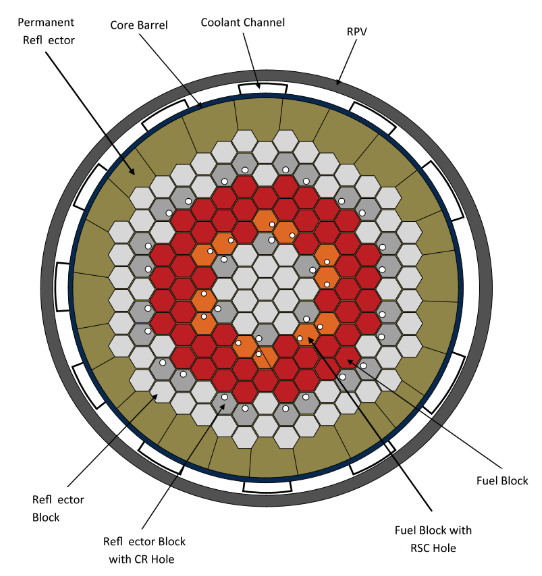
\includegraphics[width=\linewidth]{figures/radial-layout.png}
	% 		\caption{XY-plane.}
	% 	\end{subfigure}
	% 	\begin{subfigure}[t]{0.4\textwidth}
	% 		\centering
	% 		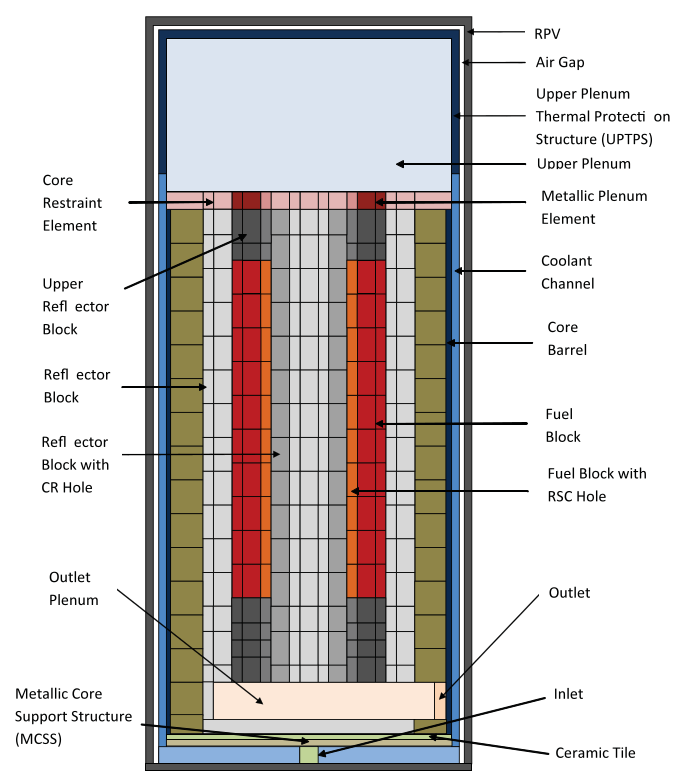
\includegraphics[width=\linewidth]{figures/axial-layout.png}
	% 		\caption{YZ-plane.}
	% 	\end{subfigure}
	% 	\hfill
	% 	\caption{MHTGR reactor layout.}
	% 	\label{fig:layout}
	% \end{figure}

	% \begin{figure}[htbp!]
	% 	\centering
	% 	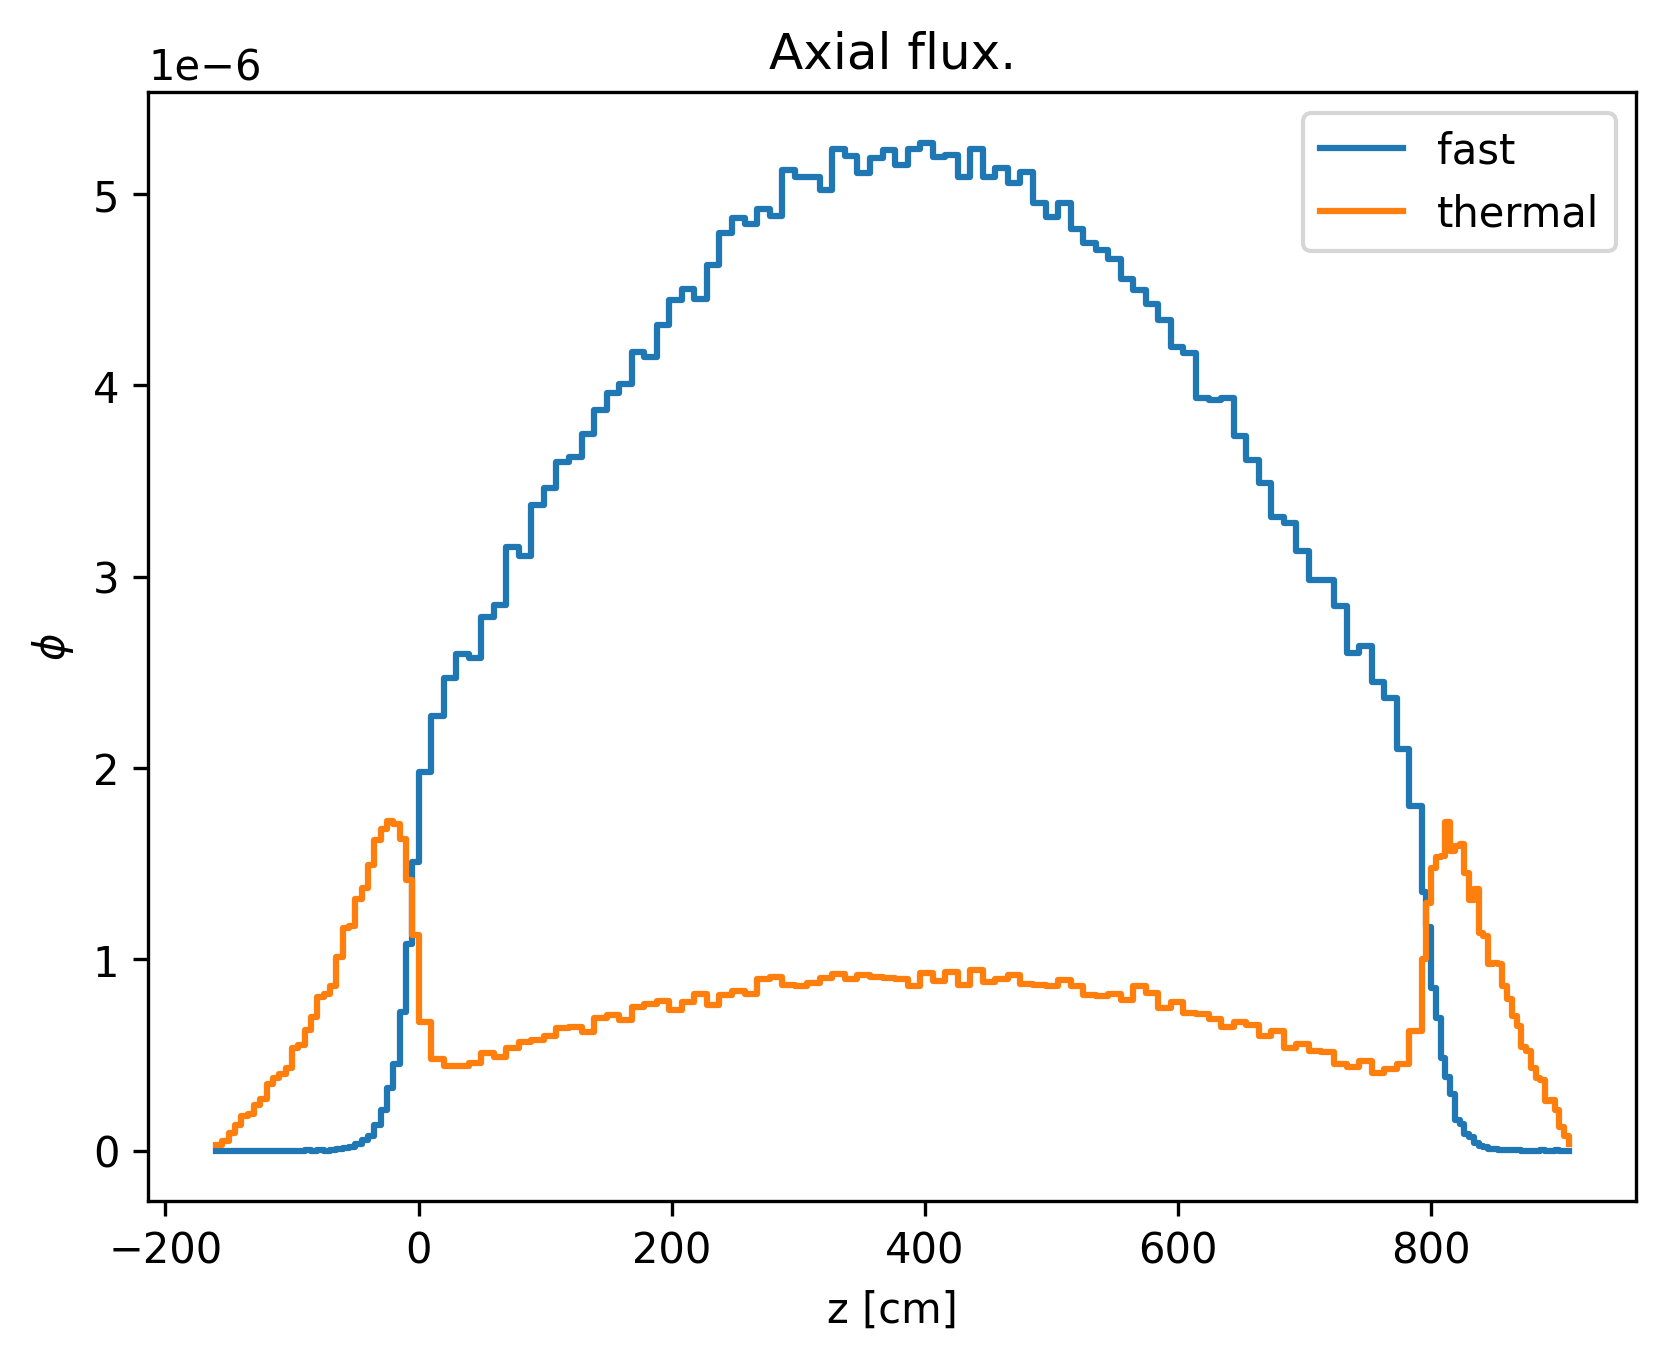
\includegraphics[width=0.6\linewidth]{figures/axial1.png}
	% 	\hfill
	% 	\caption{Neutron flux on the specified fuel channel.}
	% 	\label{fig:axial}
	% \end{figure}
